\section{Methodology}
\label{sec:methodology}


The following is the class diagram for our implementation: Figure \ref{fig:class-diagram}

\begin{figure}[h]
	\centering
	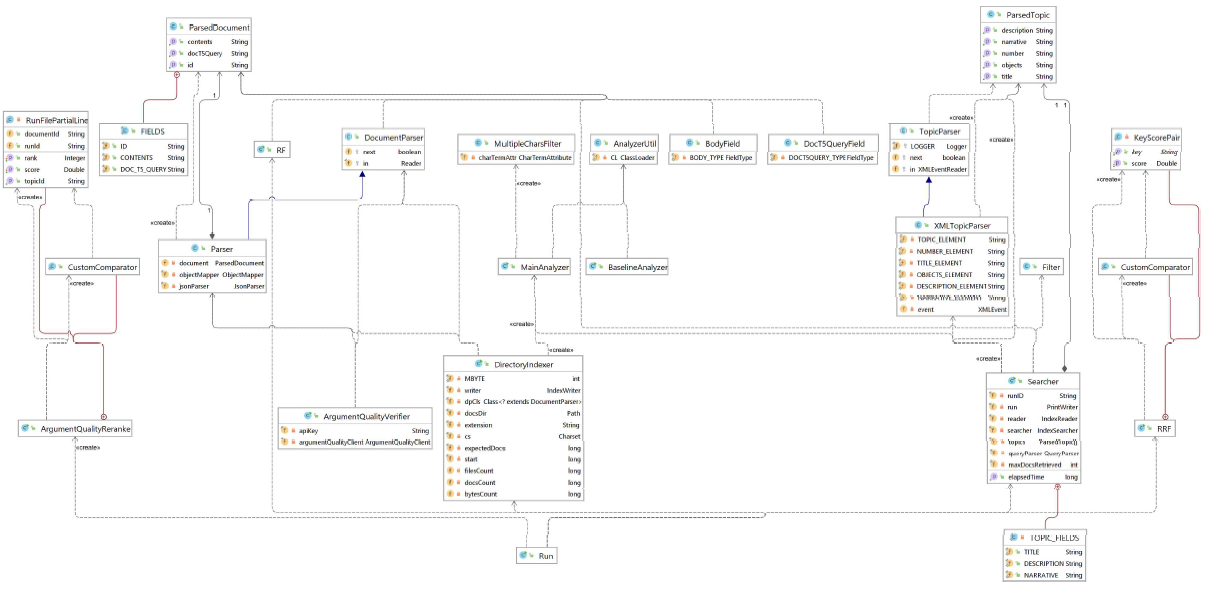
\includegraphics[width=\textwidth]{figure/class-diagram.PNG}
	\caption{Class diagram of the project}
	\label{fig:class-diagram}
\end{figure}

The developed Java system is divided into the following packages, each package representing a stage:


\subsection{Parse}
  
  This package is divided into two packages: 
\subsubsection{Document}
        
            The aim of this package of the project is to facilitate the parsing of the document corpus provided by CLEF for the Touchè Task 2 so that they can be used together with Lucene. The corpus for Task 2 is a collection of about 0.9 million text passages contained in a single JSON file passages.json. The file contains several documents organized as nodes of a JSON tree and each node contains 3 different fields. Namely id, contents, and chatNoirUrl. In this project only the id and the contents data of the document are retrieved from the JSON node and used in the implementation. The chatNoirUrl is not taken into account since we found it to not be relevant for the task. Furthermore, CLEF also provided a version of the corpus with text passages expanded with queries generated using DocT5Query. We found this expanded version valuable and added support for parsing it in our implementation. The DocT5Query queries are contained within the 'contents' key of each document. The parsing is implemented in the following classes:
            \begin{enumerate}
                \item 
                    DocumentParser.java: Similar to HelloTiptster’s, the class creates a     document parser that takes a reader object to be used as input, it overrides the hasNext() and next() methods, and performs the actual parsing.
                \item 
                    Parser.java: This is a customized class that specializes the HelloTipster parser used on the TIPSTER corpus by our teacher. It extends the aforementioned DocumentParser class and takes the reader object as input. The hasNext() method has been implemented and it is where the actual parsing takes place and it extracts the three already mentioned fields.
                \item
                    ParsedDocument.java: Represents the actual document to be indexed by Lucene. It defines the id, contents, and docT5Query of the JSON documents. The class defines proper getter and setter methods for the various fields to be easily retrieved and set, and it overrides utility methods like toString(), equals(), and hashCode().
            \end{enumerate}
\subsubsection{Topic}
        
            The aim of this package of the project is to facilitate the parsing of the topics provided by CLEF for the Touchè Task 2 so that they can be used together with Lucene. The topics of Task 2 is a collection of 50 topics contained in a single XML file topics-task2.xml. The file contains the topics each having 5 different attributes. Namely number, title, objects, description, and narrative. In this project, even though all the attributes of a topic are parsed, Only the number, objects, and title are used for search. The narrative and description attributes are used for manual relevance. The parsing is implemented in the following classes:
            \begin{enumerate}
                \item 
                    TopicParser.java: Similar to DocumentParser.java, the class creates a     topic parser that takes a reader object to be used as input, it overrides the hasNext() and next() methods, and performs the actual parsing.
                \item 
                    XMLTopicParser.java: This is a customized class that  extends the aforementioned TopicParser class and takes the reader object as input. The hasNext() method has been implemented and it is where the actual parsing takes place and it extracts the already mentioned fields.
                \item
                    ParsedTopic.java: Represents the actual topic to be used in the searcher with Lucene. It defines all the attributes of a topic. The class also defines proper getter and setter methods for the various fields to be easily retrieved and set, and it overrides utility methods like toString(), equals(), and hashCode().
            \end{enumerate}
\subsection{Analyze}
  
    We have built three analyzers, to process the documents, perform tokenization and use different combination of filters.
\subsubsection{AnalyzerUtil.java}
            
            This is a helper class auxiliary class containing utility methods for loading stop lists in the resource folder. These stop lists were obtained from well-known standard lists based off high frequency words. Some of them are: Atire, Indri, Smart, Terrier, Zettair, Glasgow, Snowball, Okapi, and Lucene. 
\subsubsection{BaselineAnalyzer.java}
            
            This is a java class for tokenization which starts with a StandardTokenizer and reduces every word to lower case using a LowerCaseFilter and then we have used the StopFilter to remove frequent words in the collection that do not bring useful information. 
\subsubsection{MainAnalyzer.java}
            
            Contains various filters from AnalyzerUtil as well as EnglishPossessiveFilter and MultipleCharsFilter. It also adds synonyms dictionary to perform a query expansion based on Wordnet.
\subsection{Index}
  
     This package contains the 3 classes responsible for the index creation, they are as follows: 
     
\subsubsection{BodyField.java}
    
        Represents the body of a specific document it has two different constructors, one accept a Reader and the other accept a String value. The only field is BODY\_TYPE  which is tokenized and not stored, keeping only document ids and term frequencies in order to minimize the space occupation. 
\subsubsection{DirectoryIndexer.java}
    
        It's used for indexing the whole directory tree, it takes as parameter the Analyzer to be used, the Similarity, the size in megabytes of the buffer for indexing documents, the directory where to store the index, the directory from which documents have to be read, the extension of the files to be indexed, the charset used for encoding documents, the total number of documents expected to be indexed and the class of the DocumentParser to be used. The constructor take these handles several exception that may rise and take care of the index writer configuration. For testing purposes we added a main method which create a new DirectoryIndexer using custom parameters and than run the method index which do the actual indexing of the documents and skip every file which doesn't have the correct extension, important to note the fact that we added a new custom parameter DocT5QueryField. 
\subsubsection{DocT5QueryField.java}
    
        It manages the new tokenized and not stored field for the document, differently from the body field this class has only one constructor which accepts Strings.
\subsection{Search}
  
  The search package contains just the Searcher class. This class is responsible for:
    \begin{enumerate}
    	\item Retrieving and preparing the topics for the search.
    	
    	The topics are retrieved directly from the topics file and parsed using the XMLTopicParser class.
    	Then an Analyzer is defined to tokenize and filter the tokens before the search.
    	\item Defining how to use topics in the search.
    	
    	We decided to use just the topics titles in the search by similarity, but we used the topic objects (the items which the user wants to compare) as a filter: we selected among the search results just the documents that presented both the terms.
    	Moreover we made it possible to assign weights to the different fields of the documents among which to search, or to select just one of the two fields (Contents and DocT5Query).
    	\item Defining which type of comparison to perform between topics and documents.
    	
    	The searcher class accepts as a parameter a similarity function to compare the two.
    	\item Writing the results on a file
    \end{enumerate}

    We experimented with different configurations. We especially tried changing:
    \begin{itemize}
    	\item Similarity functions
    	\item Whether we applied filtering or not to the search results
    	\item Analyzer, in particular the stoplist it uses
    \end{itemize}
\subsection{RF}
  
      This package contains a single class, also called RF.
        
        RF.java is a customized class with the goal of performing a search using relevance feedback to perform query expansion.
        
        RF functions in a similar way to the Searcher class, with the exception of building the query used in the searching using the tokens present in relevant documents, instead of using the terms in title field of the topics file.
        
        The class collects all docID and relevance of relevant documents in the \textit{qrels} file.
        
        The tokens and their frequency in the relevant documents are retrieved by searching the document by docID and iterating through its termvector.
        
        The tokens used in the search are boosted by their frequency in the document multiplied by the square of the relevance score.
        
        Relevance Feedback is standardly based on the Rocchio Algorithm.
        The formula for the Rocchio Algorithm is:
        $$
        \overrightarrow{Q_{m}}=
        \left(a\cdot\overrightarrow{Q_{O}}\right)+
        \left(b\cdot\frac{1}{|D_{r}|}\cdot\sum_{\overrightarrow{D_{j}}\in D_{r}}\overrightarrow{D_{j}}\right)-
        \left(c\cdot\frac{1}{|D_{nr}|}\cdot\sum_{\overrightarrow{D_{k}}\in D_{nr}}\overrightarrow{D_{k}}\right)
        $$
        where $\overrightarrow{Q_{m}}$ is the modified query vector, $\overrightarrow{Q_{O}}$ is the original query vector, $\overrightarrow{D_{i}}$ is the document vector for the $i^{th}$ document, $D_{r}$ is the set of relevant documents, $D_{nr}$ is the set of non-relevant documents and $a$, $b$ and $c$ are weight parameters.
        
        In our case the parameters used are 0, 1, 0.
        Rocchio algorithm is written for binary relevance, our version of RF is customized to take into account the different relevance scores used in this test collections (0 to 3).
        
        The results of the search are then outputted as a standard run file.
        
\subsection{RRF}
  
      This package contains a single class, also called RRF.
        
        RRF.java is a customized class with the goal of performing using Reciprocal Ranking Fusion to fuse the results of different runs in a single one.
        
        RRF takes in imput a directory path and performs RRF using all the runs in .txt documents inside that directory.
        
        For each documents and for each topic the documents and their respective ranking are collected.
        
        Then document receive a new scoring using the RRF formula.
        
        Given a set of documents \textit{D} and a set of rankings \textit{R} for the documents, the formula for RRF is:
        $$RRFscore(d \in D)=\sum_{r \in R}^{}\frac{1}{k+r(d)}$$
        where k is a fixed number, in this case k is set to 30.
        
        Then, for each topic, documents are ranked (and ordered) based on their RRF score.
        
        The results of the search are then outputted as a standard run file.
\subsection{Filter}
 
    The main filter class contains two methods responsible for adding the term to the search object. The main method is filterAnd. It takes two parameters as input: a query parser object to convert the string into a meaningful term for the search method. And a String s that represents the term that needed to add to the query parser. It will return an object of BooleanQuery.Builder which can be consumed later by the search method. The second method is just a helper method to extract the string object from the "objects field", tokenize the sentences, and remove any unwanted characters.

\subsection{Argument quality}
  \label{subsec:Argument quality}
  We decided to make use of IBM Project Debater API.
  
      Project Debater is an AI system used to perform various tasks about debating at a human level. IBM makes freely available, for research purposes, some services based on this system through an API. \citep{ProjectDebaterAPI}
      
      We were interested in the argument quality service of the API. It accepts a couple of strings labeled as Sentence and Topic, and it returns a float score in the range 0-1 based on the relevance of the sentence for the topic and on the quality of the sentence as a text, which means how good it is written. We were not interested in the first part of the evaluation because the rest of our system was designed to do that, so it would be redundant. We just wanted to evaluate the text quality. So we decided to send Sentence-Topic pairs in which the Topic part was an empty string.
      
      We coded the ArgumentQualityVerifier class which evaluates the written quality of each document by using the API and then saves the scores to a file.
      
      Then we had to use the obtained scores to rerank the results of the search saved in a run file. So we defined the ArgumentQualityReranker class which:
      
       \begin{enumerate} 
           \item loads the quality scores of all the documents from the file into a Map object \item iterates over the lines of the old run file and for each: multiplies the old score by the one assigned by Project Debater API and saves the object representing the new line to a list \item sorts the list of new lines by topic number and score and writes them on a new run file 
       \end{enumerate}

\subsection{Run.java}

The developed Java system also contains the class Run.java. This is the main class used for running the entire system. It accepts the following parameters: 

    \begin{enumerate}
        \item Task
            
            Specifies which stage to be run.
            
            Possible values: 'parse', 'index', or 'search'.
    
            Default value = 'index'
        \item indexDirectoryPath
            
            Specifies the location of index files.
            
            Possible values: the path to the index.
            
            Default value = 'experiment/index'
            
        \item stopListFilePath
            
            Specifies the location of the stop list file to use.
        
            Possible values: the path to the stop list file to be used.
            
            Default value = 'lucene.txt'
        \item filter
            
            Specifies whether or not to filter by topic objects during search
            
            Possible values: 'true', 'false'.
            
            Default value = 'false'
        \item matching
            
            Specifies the type of similarity to use.
            
            Possible values: 'bm25', 'tfidf', 'lmd'.
            
            Default value = 'bm25'
        \item runId
            
            Specifies the ID of the run.
            
            Possible values: any string.
            
            Default value = 'seupd2122-kueri'
        \item runDirectoryPath
            
            Specifies the directory  to which to write runs.
            
            Possible values: any valid directory path.
            
            Default value = 'runs'
        \item qrelFilePath
            
            Specifies the directory to which to write qrels of RF search.
            
            Possible values: any valid directory path.
            
            Default value = 'code/src/main/resource/qrels/example.txt'

\end{enumerate}